%%
%% This is file `sample-sigplan.tex',
%% generated with the docstrip utility.
%%
%% The original source files were:
%%
%% samples.dtx  (with options: `sigplan')
%% 
%% IMPORTANT NOTICE:
%% 
%% For the copyright see the source file.
%% 
%% Any modified versions of this file must be renamed
%% with new filenames distinct from sample-sigplan.tex.
%% 
%% For distribution of the original source see the terms
%% for copying and modification in the file samples.dtx.
%% 
%% This generated file may be distributed as long as the
%% original source files, as listed above, are part of the
%% same distribution. (The sources need not necessarily be
%% in the same archive or directory.)
%%
%% Commands for TeXCount
%TC:macro \cite [option:text,text]
%TC:macro \citep [option:text,text]
%TC:macro \citet [option:text,text]
%TC:envir table 0 1
%TC:envir table* 0 1
%TC:envir tabular [ignore] word
%TC:envir displaymath 0 word
%TC:envir math 0 word
%TC:envir comment 0 0
%%
%%
%% The first command in your LaTeX source must be the \documentclass command.
\documentclass[sigplan,screen]{acmart}
%% NOTE that a single column version is required for 
%% submission and peer review. This can be done by changing
%% the \doucmentclass[...]{acmart} in this template to 
%% \documentclass[manuscript,screen,review]{acmart}
%% 
%% To ensure 100% compatibility, please check the white list of
%% approved LaTeX packages to be used with the Master Article Template at
%% https://www.acm.org/publications/taps/whitelist-of-latex-packages 
%% before creating your document. The white list page provides 
%% information on how to submit additional LaTeX packages for 
%% review and adoption.
%% Fonts used in the template cannot be substituted; margin 
%% adjustments are not allowed.
%%
%% \BibTeX command to typeset BibTeX logo in the docs
\AtBeginDocument{%
  \providecommand\BibTeX{{%
    \normalfont B\kern-0.5em{\scshape i\kern-0.25em b}\kern-0.8em\TeX}}}

%% Rights management information.  This information is sent to you
%% when you complete the rights form.  These commands have SAMPLE
%% values in them; it is your responsibility as an author to replace
%% the commands and values with those provided to you when you
%% complete the rights form.
\setcopyright{acmcopyright}
\copyrightyear{2018}
\acmYear{2018}
\acmDOI{XXXXXXX.XXXXXXX}

%% These commands are for a PROCEEDINGS abstract or paper.
\acmConference[Conference acronym 'XX]{Make sure to enter the correct
  conference title from your rights confirmation emai}{June 03--05,
  2018}{Woodstock, NY}
%
%  Uncomment \acmBooktitle if th title of the proceedings is different
%  from ``Proceedings of ...''!
%
%\acmBooktitle{Woodstock '18: ACM Symposium on Neural Gaze Detection,
%  June 03--05, 2018, Woodstock, NY} 
\acmPrice{15.00}
\acmISBN{978-1-4503-XXXX-X/18/06}


%%
%% Submission ID.
%% Use this when submitting an article to a sponsored event. You'll
%% receive a unique submission ID from the organizers
%% of the event, and this ID should be used as the parameter to this command.
%%\acmSubmissionID{123-A56-BU3}

%%
%% The majority of ACM publications use numbered citations and
%% references.  The command \citestyle{authoryear} switches to the
%% "author year" style.
%%
%% If you are preparing content for an event
%% sponsored by ACM SIGGRAPH, you must use the "author year" style of
%% citations and references.
%% Uncommenting
%% the next command will enable that style.
%%\citestyle{acmauthoryear}

%%
%% end of the preamble, start of the body of the document source.
\begin{document}

%%
%% The "title" command has an optional parameter,
%% allowing the author to define a "short title" to be used in page headers.
\title{Trabalho Prático - IA}

%%
%% The "author" command and its associated commands are used to define
%% the authors and their affiliations.
%% Of note is the shared affiliation of the first two authors, and the
%% "authornote" and "authornotemark" commands
%% used to denote shared contribution to the research.
\author{Eric Azevedo de Oliveira}
\affiliation{%
 %% \institution{The Th{\o}rv{\"a}ld Group}
 %% \streetaddress{1 Th{\o}rv{\"a}ld Circle}
  \city{Belo Horizonte}
  \country{Brasil}}
\email{eric.azevedo@sga.pucminas.br}

\author{Felipe Nepomuceno Coelho}
\affiliation{%
 %% \institution{The Th{\o}rv{\"a}ld Group}
  %%\streetaddress{1 Th{\o}rv{\"a}ld Circle}
  \city{Belo Horizonte}
  \country{Brasil}}
\email{felipe.coelho.1265277@sga.pucminas.br}



\author{Iyan Lucas Duarte Marques}
\affiliation{%
 %%\institution{Rajiv Gandhi University}
%% \streetaddress{Rono-Hills}
 \city{Belo Horizonte}
 \country{Brasil}}
\email{ildmarques@sga.pucminas.br}


%%
%% By default, the full list of authors will be used in the page
%% headers. Often, this list is too long, and will overlap
%% other information printed in the page headers. This command allows
%% the author to define a more concise list
%% of authors' names for this purpose.
%%\renewcommand{\shortauthors}{Trovato and Tobin, et al.}

%%
%% The abstract is a short summary of the work to be presented in the
%% article.



%%
%% The code below is generated by the tool at http://dl.acm.org/ccs.cfm.
%% Please copy and paste the code instead of the example below.




%%
%% Keywords. The author(s) should pick words that accurately describe
%% the work being presented. Separate the keywords with commas.


%% A "teaser" image appears between the author and affiliation
%% information and the body of the document, and typically spans the
%% page.


%%
%% This command processes the author and affiliation and title
%% information and builds the first part of the formatted document.
\maketitle


\begin{figure}[h]
  \centering
  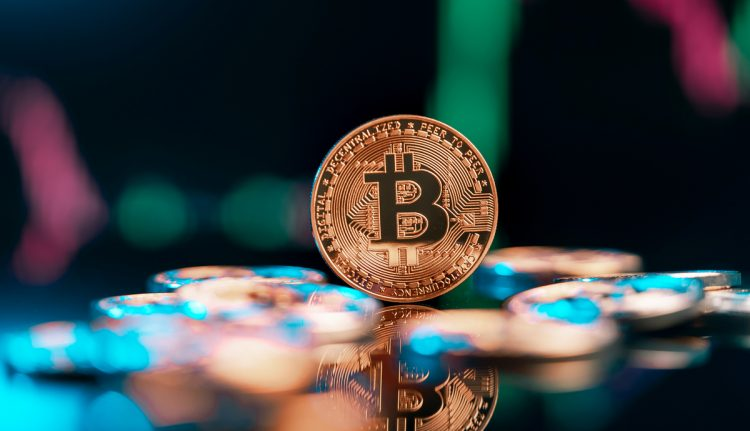
\includegraphics[width=\linewidth]{btc.jpg}
  \caption{Estudantes em sala de aula, realizando provas. (\url{https://medium.com/@JaskySingh/what-if-we-had-exams-everyday-well-everyone-would-be-better-off-f97919edeac}).}
  \Description{Estudantes em dia de prova.}
\end{figure}



\section{Introduction}
A base a ser utilizada será a "Bitcoin Historical Data" que pode ser encontrada em \url{https://www.kaggle.com/datasets/mczielinski/bitcoin-historical-data}.
A base é composta por 8 atributos, sendo eles nominais, binários e numéricos:
\begin{itemize}
    \item Timestamp - A data da instância (UNIX Timestamp) 
    \item Open - Preço da abertura do Bitcoin no início do pregão
    \item High - Teto do preço do Bitcoin do pregão
    \item Low - Piso do preço do Bitcoin do pregão
    \item Close - Preço do fechamento do Bitcoin no término do pregão
    \item Volume\_(BTC) - Volume de Bitcoins transacionado no pregão
    \item Volume\_(Currency) - Volume de outras moedas transacionado no pregão\footnote{Moedas convertidas para BTC, como Real para BTC}
    \item Weighted\_Price - \textit{VWAP- Volume Weighted Average Price}
\end{itemize}

A base "Bitcoin Historical Data" possui 4857378 instâncias e é um problema de predição e apresenta o histórico de preço da moeda, desde 2012 a janeiro de 2021.

\section{Related Works}
Moedas outras formas de pagamento são utilizadas desde 2200 AC, agora na era da informação, estamos digitalizando esta forma milenar de relações interpessoais.
Desta forma, abaixo estão apresentados trabalhos a respeito deste tema, bem como os conceitos das criptomoeda e o bitcoin, além das suas implicações nos governos e cotidiano:

As criptomoedas e as suas tecnologias como blockchain contrastaram com os métodos tradicionais, as moedas fiduciárias\footnote{
  Moeda fiduciária é qualquer título não-conversível, ou seja, não é lastreado a nenhum metal (ouro, prata) e não tem nenhum valor intrínseco.\cite{lara2008estudo}
}. 
como dito no artigo\cite{8567098}, os autores discorrem sobre as diferenças entre as criptomoedas e as moedas \textit{fiat}. 
Uma das diferenças mostradas por eles são por exemplo: o modelo as quais ambas foram arquitetadas.
No qual o portador da moeda fiat, através um dos seus vetores o cartões de credito, realiza uma transação que é rastreada da sua origem para o seu destino.
Já as criptomoedas, são projetadas com a finalidade do anonimato e privacidade, de forma a não ser possível identificar a origem e nem os rastreio das mesmas.

Já no artigo \cite{ADMREV2413}, os autores iniciam a discussão contextualizando como surgiu a moeda, referenciando seu contexto histórico e fazendo comparações com o passado.
Logo em seguida, é especificado que as moedas virtuais vem crescendo nos últimos tempos por vários motivos como: a não regularização da moeda, diminuindo assim o monopólio governamental, o sigilo por parte dos negociantes, o valor da moeda ser flutuante, entre outras vantagens.
Neste contexto os autores ampliam a discussão mostrando que a descentralização do Bitcoin é um passo fundamental e um catalisador de um novo modelo econômico.
Modelo esse que não necessita de uma figura estatal como controladora e mediadora para se obter um sistema econômico que permita as transações.

Se aprofundando mais no quesito da flutuabilidade, o maior atrativo para investidores e a movimentação de capital em pregões, de acordo com \cite{UMAR2021121025}, uma das maiores diferenças entre os tipos de moeda, as criptomoedas são bem mais voláteis em relação às tradicionais.
Não só isso, mas o impacto de eventos como o coronavirus e as coberturas midiáticas afetam a moeda virtual de forma bem mais incisiva. 
Concluindo com as comparações das flutuações cambiárias no período da pandemia, e um pequeno briefing de períodos bem notáveis.

O artigo \cite{dos2021cenario}, tem como objetivo: fazer uma análise sobre as influências do cenário e perspectiva da criptomoeda Bitcoin no contexto econômico e social brasileiro.
Criptomoedas são códigos virtuais valorados por seu custo físico e sua flutuação dentro de um cenário financeiro próprio e decentralizado, mas que possuem a possibilidade de venda e troca por produtos tanto digitais quanto moedas fiduciárias.
Argumentando ser externa a cotação de moedas fortes e já existentes como o dólar, o autor fala de como o bitcoin se tornou uma ótima alternativa de investimento, ainda mais em contextos de crises globais.
Apresentando a ideia de sua criação, a ausência de um órgão regulador e a rede Blockchain, eles apresentam um potencial democrático de investimento na moeda, dando acesso a um valor de compra de, por exemplo, 1\$ e ainda obter lucros consideráveis.

No \cite{8323676} o autor mostra 2 modelos de predição sobre o preço da criptomoeda bitcoin.
O primeiro modelo realizava uma predição, utilizando GLM/Random Forest, direta ao valor da moeda, o mesmo que teve uma taxa de erro e desvio alta.
O segundo Modelo trouxe uma estratégia um pouco diferente, sua predição é baseada na tendência de subida/queda da moeda, mediante a utilização de uma rede neural artificial, dessa forma esse modelo foi capaz de atingir 79\% de acurácia se mostrando efetivo.
Em uma terceira análise, são comparados Multi-Layer Perceptron (MLP) e Non-linear auto-regressive exogenous (NARX), sendo concluído que o MLP pode ser utilizado para predição, entretanto sem superar o NARX.
O autor também ressalta o impacto da normalização dos dados utilizando 5 técnicas, sendo elas Log Normalization, In built MATLAB method, Standard deviation normalization, Z score normalization, Boxcox normalization.
Embora os resultados sejam individuais, todas as técnicas levaram a uma melhora significativa à acurácia.   
%-----------------------------------------------------------
% COLOCAR ESSA PARTE SOMENTE SE JULGAR NECESSÁRIO

% Buscando a melhor forma de resolver o problema da predição do bitcoin, o estudo demonstra a aplicação de algumas técnicas de pré-processamento em duas bases relacionadas à variação do bitcoin, demostrando a melhora na acurácia e propõe um novo estudo em que será utilizada a Regressão Bayesiana e o GLM/Random Forest para a resolução de tal problemática.

%------------------------------------------------
%% Forma de  \cite{Ablamowicz07}





%%
%% The next two lines define the bibliography style to be used, and
%% the bibliography file.

\bibliographystyle{ACM-Reference-Format}
\bibliography{sample-base}

%%
%% If your work has an appendix, this is the place to put it.


\end{document}
\endinput
%%
%% End of file `sample-sigplan.tex'.
